%% twi_desc.ltx
%%

\documentclass{article}
\usepackage{times}
%\usepackage{amsmath}
%\usepackage{epsfig}
\usepackage{graphicx}
\usepackage{tikz}
%\usepackage{tikzscale}
\usetikzlibrary{shapes,calc,positioning}
\usetikzlibrary{arrows.meta,bending}
\usepackage{tikz-timing}
%\usetikztiminglibrary[rising arrows]{clockarrows}

\setlength{\topmargin}{-.5in}
\setlength{\textheight}{9in}
\setlength{\textwidth}{6.5in}
\setlength{\evensidemargin}{0in}
\setlength{\oddsidemargin}{0in}

\title{%
Notes on Using TWI for AVR 0-series MCUs
}
\author{MattRW}
\date{\large 11 Jan 2020}

\newcommand{\uA}{\ensuremath{\!\uparrow}}
\newcommand{\dA}{\ensuremath{\!\downarrow}}
\newcommand{\udA}{\ensuremath{\!\updownarrow}}
\newcommand{\ua}{\ensuremath{\uparrow}}
\newcommand{\da}{\ensuremath{\downarrow}}
\newcommand{\uda}{\ensuremath{\updownarrow}}
\newcommand{\tF}{t\ensuremath{_F}}
\newcommand{\tH}{t\ensuremath{_H}}
\newcommand{\tL}{t\ensuremath{_L}}
\newcommand{\ti}{t\ensuremath{_1}}
\newcommand{\ra}{\ensuremath{\rightarrow}}
\newcommand{\SCL}{{\sc SCL}}
\newcommand{\SDA}{{\sc SDA}}



\begin{document}
%\maketitle

\iffalse
NOTES

The master always runs SCL.  The slave (should always) stretch.
1) TMOUT/pin_wrD(scl, 0) -> 2
2) SHIFT/wait(t_lo) -> 3
3) TMOUT/pin_wr(scl, 1) -> 1


When slave needs to change SDA, it
S) XH (SDA-SCL)
1) waits for SCL hi->lo (SHIFT)
2) pulls SCL low, pulls SDA hi/lo
3) if (2) SDA is change, wait for transition, else goto (4)
4) waits for SCL lo->hi (LATCH);
   checks SDA level if SDA commanded low, but is high, signal error
5) waits for SCL hi->lo (SHIFT), then release SDA
P) HL

\fi

%\vskip 1pc
%One byte write.

\iffalse
\begin{tabular}{|l|l|p{3in}|}
  \hline
  M start &
  $D\dA \tF \tH $ &
  start \\ \hline

  M addr x &
  $\left[\, C\dA\,\tF\,D\udA\,\ti\,C\uA\,\tH\,\right]_8 $ &
  addr, R/W \\ \hline

  S ack M &
  $ C\dA d\udA C\uA C\dA d\uA \tL $ &
  S sets Dn until M releases \\ \hline

  \iffalse
  S ack/str &
  $C\dA d\udA c\dA C\uA t_X c\uA  C\dA d\uA $ &
  S sets D, stretches SCL \\ \hline
  \fi
  
  M send &
  $C\dA D\udA \left[C\dA\,\tF\,D\udA\,\ti\,C\uA\,\tH\,?\right]_8$ &
  \\ \hline
\end{tabular}
\fi

\includegraphics[width=5.5in]{timing}
\vskip 1pc
%    timing/dslope=0.1,
%    timing/.style={x=5ex,y=2ex},
%    x=5ex,
%    timing/rowdist=3ex,
%    timing/name/.style={font=\sffamily\scriptsize}
\begin{tikztimingtable}[%
    timing/slope=1,
    timing/yunit=.8cm,timing/rowdist=1.2cm,
    timing/draw grid,
    timing/name/.style={font=\sffamily\scriptsize}
  ]
  {SDA} & HHHLLLUDDDDSSDDUDDDDDD \\
  {SCL} & HHHHHLLSLHHSSHLLSSLH \\
  %{st} & 1D{0}1D{1}1D{2}1D{3}1D{4} \\
\end{tikztimingtable}
\vfill
\vfill

%WRT transtions in a M|S event $\ua$ or $\da$ represents observation of
%the bus.  That is $>0.7V_{dd}$ or $<0.3V_{dd}$

\begin{centering}
\begin{tabular}{c@{}p{2.5cm} c@{}p{2cm} c@{}p{2cm} }
  \underline{M} & & \underline{B} & & \underline{S} & \\ 

  0  & & HH & & HH & \\
  $\da$ & $/D\dA$ & $\dA$ & $D\dA$ & $\dA$ & $D\dA/$ S\\
  \\

  1 &  & LH & & LH & \\
  $\da$ & $t_H/C\dA $ & $\dA$ & $C\dA$ & $\dA$ & $C\dA$ \\
  \\

  2 &  & LL & & LL & \\
  $\da$ & $t_F/D\udA $ & $\da$ & $D\udA$ & $\da$ & $D\udA$ \\
  \\

  3 & & xL  & & xL & \\
  $\da$ & $t_L/C\uA $ & $\da$ & $C\uA$  & $\da$ &  \\
  \\

  4 & & xR  & & xL & \\
  $\da$ & & $\da$ & $t_R/C\uA$ & $\da$ &  $C\uA/l$ \\
  \\

  5 &  & xH & & xH & \\
  $\da$ & $t_H/C\dA $ & $\da$ & $C\dA$  & $\da$ & $C\dA/s$ \\
  \\

  % the following is wrong because 3 is LL and we go to Lx
  6 & \hfil $[n>0] \ra 2$  & ?L & & ?L & \\
  $\da$ & $[n=0]$ & $\da$ &  & $\da$ & \\
  \\

  7 &  & xL & & xL & \\
  $\da$ & $D\dA/l$ & $\da$ & $D\dA$ & $\da$ & $/ D\dA$ \\
  \\

  % optional clock stretch here
  
  8 &  & LL & & LL & \\
  $\da$ & $t_L/C\uA$ & $\da$ & $C\uA$ & $\da$ &   \\
  \\

  9 &  & LR & & LL & \\
  $\da$ & $t_L/C\uA $ & $\da$ & & $\da$ & $C\uA/D\uA $ \\
  \\

  \iffalse
  10 &  & LH & & LH & \\
  $\da$ &  & $\da$ & & $\da$ & \\

  11 &  & LH & & LH & \\
  $\da$ &  & $\da$ & & $\da$ & \\

  12 &  & LH & & LH & \\
  $\da$ &  & $\da$ & & $\da$ & \\

  13 &  & LH & & LH & \\
  $\da$ &  & $\da$ & & $\da$ & \\

  14 &  & LH & & LH & \\
  $\da$ &  & $\da$ & & $\da$ & \\
  \fi

\end{tabular}
\end{centering}

\vskip 1pc
\begin{figure}[h]
  \begin{centering}
  %% mon_diag.tex - TWI bus monitor or node_mon.tex ?

% todo: MCMD for recv data, repeated start
% todo: must check ERR before DACK

% bus monitor, simple version
% : monitors  SCL, SDA state to generate START, STOP, bits
%\tikzset{>={Stealth[width=3mm,length=3mm]}}
\iftrue
\vskip 1pc
\begin{tikzpicture}%
  [text=black, node font=\small,scale=0.8]

  \node (HH) at (0,0) [circle, draw, radius=1cm] {HH};
  \node (LH) at ($(HH)+(-4cm,-4cm)$) [circle, draw, radius=1cm] {LH};
  \node (HL) at ($(HH)+(4cm,-4cm)$) [circle, draw, radius=1cm] {HL};
  \node (LL) at ($(HL)+(-4cm,-4cm)$) [circle, draw, radius=1cm] {LL};

  \node (SDA) at ($(HH)+(-4.0cm,-0.5cm)$) [rotate=45]
        {L$\longleftarrow$ SDA $\longrightarrow$H};
  \node (SCL) at ($(HH)+(4.0cm,-0.5cm)$) [rotate=-45]
        {H$\longleftarrow$ SCL $\longrightarrow$L};

  \draw[->] (HH) edge[bend left=15] node[above,sloped] {SDA \da\,/start} (LH);
  \draw[->] (LH) edge[bend left=15] node[above,sloped] {SDA \ua\,/stop} (HH);

  \draw[->] (HH) edge[bend left=15] node[above,sloped] {SCL \da\,/s} (HL);
  \draw[->] (HL) edge[bend left=15] node[above,sloped] {SCL \ua\,/l} (HH);
  
  \draw[->] (LH) edge[bend left=15] node[above,sloped] {SCL \da\,/s} (LL);
  \draw[->] (LL) edge[bend left=15] node[above,sloped] {SCL \ua\,/l} (LH);
  
  \draw[->] (HL) edge[bend left=15] node[above,sloped] {SDA \da} (LL);
  \draw[->] (LL) edge[bend left=15] node[above,sloped] {SDA \ua} (HL);

  \node (sig) [below=3.5 of LH,rectangle,draw,anchor=west]
        {\tiny simple TWI monitor};
  \node (sig) [below=3.5 of HL,rectangle,draw,anchor=east]
        {\tiny MattRW v210425a};
  
\end{tikzpicture}
\fi

% simulation model
\iffalse
\vskip 1pc
\begin{tikzpicture}[text=black,node font=\small]

  \node (HH) at (0,0) [circle, draw, radius=1cm] {HH};
  \node (HL) at ($(HH)+(4cm,-4cm)$) [circle, draw, radius=1cm] {HL};
  \node (LH) at ($(HH)+(-4cm,-4cm)$) [circle, draw, radius=1cm] {LH};
  \node (LL) at ($(LH)+(4cm,-4cm)$) [circle, draw, radius=1cm] {LL};
  \node (RH) at ($0.5*(HH)+0.5*(LH)+(-0.5cm,0.5cm)$)
        [circle, draw, radius=1cm] {RH};
  \node (RL) at ($0.5*(HL)+0.5*(LL)+(-0.5cm,0.5cm)$)
        [circle, draw, radius=1cm] {RL};

  \node (SCL) at ($(HH)+(-4.0cm,-0.5cm)$) [rotate=45]
        {L$\longleftarrow$ SCL $\longrightarrow$H};
  \node (SDA) at ($(HH)+(4.0cm,-0.5cm)$) [rotate=-45]
        {H$\longleftarrow$ SDA $\longrightarrow$L};

  \draw[->] (HH) edge[bend left=15] node[above,sloped] {[any L]/start} (HL);
  \draw[->] (HL) edge[bend left=15] node[above,sloped] {[all H]/stop} (HH);

  \draw[->] (HH) edge[bend left=15] node[above,sloped] {[any L]} (LH);
  \draw[->] (LH) edge[bend left=15] node[above,sloped] {[all H]} (RH);
  \draw[->] (RH) edge[bend left=15] node[above,sloped] {} (HH);
  
  \draw[->] (HL) edge[bend left=15] node[above,sloped] {[any L]} (LL);
  \draw[->] (LL) edge[bend left=15] node[above,sloped] {[all H]} (RL);
  \draw[->] (RL) edge[bend left=15] node[above,sloped] {} (HL);
  
  
  \draw[->] (LH) edge[bend left=15] node[above,sloped] {[any L]/data=0} (LL);
  \draw[->] (LL) edge[bend left=15] node[above,sloped] {[all H]/data=1} (LH);
  
  %\draw[->] (HH) edge[out=90,in=0,looseness=8] node[right,pos=0.4] {} (HH);
  %\draw[->] (HL) edge[out=45,in=-45,looseness=8] node[right] {} (HL);

  \node (sig) [below=3.5 of LH,rectangle,draw,anchor=west]
        {\tiny simulation model};
  \node (sig) [below=3.5 of HL,rectangle,draw,anchor=east]
        {\tiny MattRW v210218a};
  
\end{tikzpicture}
\fi

% --- last line ---

  \end{centering}
\end{figure}

\vfill

\iffalse

This document reflects work-in-progress on working with TWI on the
0-series of AVR microcontrollers.  My first project will be to retrive
data from an I2C based M6040(???) based IMU.

MSTATUS:\hfil\break
\begin{tabular}{r|c|c|c|c|c|c|c|c|}
 bit & 7 & 6 & 5 & 4 & 3 & 2 & 1 & 0 \\
     & RIF & WIF & HOLD & ACK & ARBLOST & ERR & \multicolumn{2}{|c|}{STATE} \\
     &  RW & RW & RW & R & RW & RW & RW & RW
\end{tabular}

SSTATUS:\hfil\break
\begin{tabular}{r|c|c|c|c|c|c|c|c|}
 bit & 7 & 6 & 5 & 4 & 3 & 2 & 1 & 0 \\
     & DIF & APIF & HOLD & RXACK & COL & ERR & DIR & AP \\
     &  RW & RW & R & R & RW & RW & R & R
\end{tabular}

\begin{figure}[h]\label{fig:1}
  \centering
  % todo: MCMD for recv data, repeated start
% todo: must check ERR before DACK
\begin{tikzpicture}[%
    text=black,
    node font=\small,
    >=stealth,
    arrow/.style={scale=2}]

  %
  \node (WS2) at (0,0) [rectangle, rounded corners=15pt,
    draw, minimum height=0.4in, minimum width=0.75in, thick]
        {\parbox[c]{1.0in}{\centering{WAIT for Wr ADDR SENT}}};
  \node (WD3a) [right=2.5cm of WS2, diamond, draw] {};
  \node (WD3b) [right=0cm of WD3a, diamond, draw] {};
  \node (WD3c) [right=0cm of WD3b, diamond, draw] {};
  \node (WD4) [right=1.8cm of WD3c, diamond, draw] {};
  \node (WS5) [right=2.5cm of WD4, rectangle, rounded corners=15pt, draw,
    minimum height=0.4in, minimum width=0.7in, thick]
        {\parbox[t]{0.9in}{\centering{WAIT for DATA SENT}}};
  \node (WD6a) [right=2.5cm of WS5, diamond, draw ] {};
  \node (WD6b) [right=0cm of WD6a, diamond, draw ] {};

  \node (S1) at ($(WD4)+(0,-3.0cm)$) [rectangle, rounded corners=15pt, draw,
    minimum height=0.4in, minimum width=0.8in, thick]
        {\parbox[t]{0.6in}{\centering{\bf READY}}};
  %
  \node (S0) at ($(S1.north)+(-1.0cm,0.5cm)$)
        [circle, draw, radius=8pt, fill] {};
  \draw[->] (S0) -- (S1);

  % new:
  \node (FAIL) at ($(S1)+(8.0cm,0)$) [rectangle, rounded corners=15pt, draw,
    minimum height=0.4in, minimum width=0.8in, thick]
        {\parbox[t]{0.6in}{\centering{\bf FAIL}}};
  % ^new
  \draw[->] (FAIL.west) -- node[above] {50:reset/reset} (S1.east);

  \draw[->] (S1.165) --
  node[below,pos=0.3,sloped] {11:\textbf{write}/addr} (WS2);

  \draw[->] (WS2.east) -- node[above] {12:intr[WIF]} (WD3a.west);
  \draw[->] (WD3c.east) -- node[above] {14:[ACK]} (WD4.west);
  \draw[->] (WD4.east) -- node[above,pos=0.4] {16:[nw$>$0]/put} (WS5.west);
  \draw[->] (WS5.east) -- node[above,pos=0.5] {20:intr[WIF]} (WD6a.west);
  \draw[->,rounded corners] (WD6b.north) --
     node[right,pos=0.3] {22:[ACK]/nw-{}-} ($(WD6b)+(0,1cm)$)
     -- ($(WD4)+(0,1cm)$) -- (WD4.north);
  %
  \node (WD7) [below=0.5cm of WD4, diamond, draw] {};
  \draw[->] (WD4.south) -- node[right,pos=0.5] {17:[nw=0]} (WD7.north);
  \draw[->] (WD7.south) -- node[right,pos=0.2] {18:[else]/stop} (S1.north);

  \coordinate (t15S) at (WD3c.north);
  \coordinate (t15E) at (FAIL.15);
  \coordinate (t15a) at ($(t15S)+(0,1.5cm)$);
  \coordinate (t15b) at ($(t15a)+(13.0cm,0)$);
  \coordinate (t15c) at ($(t15b)+(0,-3.5cm)$);
  \draw[->,rounded corners] (t15S) -- (t15a) --
            node[above,sloped] {15:[NACK]/stop} (t15b) -- (t15c) -- (t15E);

  \coordinate (t13S) at (WD3b.north);
  \coordinate (t13E) at (FAIL.10);
  \coordinate (t13a) at ($(t13S)+(0,2.0cm)$);
  \coordinate (t13b) at ($(t13a)+(13.75cm,0)$);
  \coordinate (t13c) at ($(t13b)+(0,-4.25cm)$);
  \draw[->,rounded corners] (t13S) -- (t13a) --
            node[above,sloped] {13:[BUSERR]/reset?} (t13b) -- (t13c) -- (t13E);

  \coordinate (t24S) at (WD3a.north);
  \coordinate (t24E) at (FAIL.5);
  \coordinate (t24x25) at (t24S |- t15a);
  %\node[diamond,draw] (d24x25) at (t24x25) {X};
  \coordinate (t24a) at ($(t24S)+(0,2.5cm)$);
  \coordinate (t24b) at ($(t24a)+(14.5cm,0)$);
  \coordinate (t24c) at ($(t24b)+(0,-5.0cm)$);
  \draw[->,rounded corners] (t24S) -- (t24x25) -- (t24a) --
     node[above] {24:[ARBLOST]/?} (t24b) -- (t24c) -- (t24E);

  %\coordinate (t25S) at (d24x25.west);
  %\coordinate (t25E) at (WS2.north);
  %\coordinate (t25a) at (t25S -| t25E);
  %\draw[->,rounded corners] (t25S) -- node[above] {25:[nwr$>$0]/nwr-{}-,addr} 
  %(t25a) -- (t25E);

  \coordinate (t21S) at (WD6a.south);
  \coordinate (t21E) at (FAIL.north -| t21S);
  \draw[->] (t21S) -- node[left] {21:[BUSERR]/reset} (t21E);
  
  \coordinate (t23S) at (WD6b.south);
  \coordinate (t23E) at (FAIL.north -| t23S);
  \draw[->] (t23S) -- node[right] {23:[NACK]/stop} (t23E);

  % ============================================================================
  
  \node (RD4) at ($(S1)+(0,-3.0)$) [diamond,draw] {};
  \node (RD3c) [left=1.8cm of RD4, diamond, draw] {};
  \node (RD3b) [left=0cm of RD3c, diamond, draw] {};
  \node (RD3a) [left=0cm of RD3b, diamond, draw] {};
  \node (RS2) [left=2.5cm of RD3a, rounded corners=15pt,
    draw, minimum height=0.4in, minimum width=0.75in, thick]
        {\parbox[c]{1.0in}{\centering{WAIT for Rd ADDR SENT}}};
  \node (RS5) [right=2.5cm of RD4, rectangle, rounded corners=15pt, draw,
    minimum height=0.4in, minimum width=0.7in, thick]
        {\parbox[t]{0.9in}{\centering{WAIT for DATA RCVD}}};
  \node (RD6a) [right=2.5cm of RS5, diamond, draw ] {};
  %\node (RD6b) [right=1.0cm of RD6a, diamond, draw ] {};
  \node (RD6b) [right=0cm of RD6a, diamond, draw ] {};
  
  \draw[->] (S1.195) --
  node[above,pos=0.3,sloped] {31:\textbf{read}/addr} (RS2);

  \draw[->] (RS2.east) -- node[below,pos=0.5] {32:intr[WIF]} (RD3a.west);
  \draw[->] (RD3c.east) -- node[below] {34:[ACK]} (RD4.west);
  \draw[->] (RD4.east) -- node[below,pos=0.4] {36:[nr$>$0]} (RS5.west);
  \draw[->] (RS5.east) -- node[below,pos=0.4] {40:intr[RIF]} (RD6a.west);
  %\draw[->] (RD6a.east) -- node[below] {[else]} (RD6b.west);
  \draw[->,rounded corners] (RD6b.south) --
      node[right,pos=0.3] {42:[ACK]/get,nr-{}-}
      ($(RD6b)+(0,-1cm)$) -- ($(RD4)+(0,-1cm)$) -- (RD4.south);
  %
  \node (RD7) [above=0.5cm of RD4, diamond, draw ] {};
  \draw[->] (RD4.north) -- node[right,pos=0.5] {37:[nr=0]} (RD7.south);
  \draw[->] (RD7.north) -- node[right,pos=0.2] {38:[else]/stop} (S1.south);

  \coordinate (t35S) at (RD3c.south);
  \coordinate (t35E) at (FAIL.345);
  \coordinate (t35a) at ($(t35S)+(0,-1.5cm)$);
  \coordinate (t35b) at ($(t35a)+(13.0cm,0)$);
  \coordinate (t35c) at ($(t35b)+(0,3.5cm)$);
  \draw[->,rounded corners] (t35S) -- (t35a) --
        node[below,sloped] {35:[NACK]/stop} (t35b) -- (t35c) -- (t35E);
  
  \coordinate (t33S) at (RD3b.south);
  \coordinate (t33E) at (FAIL.350);
  \coordinate (t33a) at ($(t33S)+(0,-2.0cm)$);
  \coordinate (t33b) at ($(t33a)+(13.75cm,0)$);
  \coordinate (t33c) at ($(t33b)+(0,4.25cm)$);
  \draw[->,rounded corners] (t33S) -- (t33a) --
        node[below,sloped] {33:[BUSERR]/reset} (t33b) -- (t33c) -- (t33E);
  
  \coordinate (t44S) at (RD3a.south);
  \coordinate (t44E) at (FAIL.355);
  \coordinate (t44x45) at (t44S |- t35a);
  %\node[diamond,draw] (d44x45) at (t44x45) {};
  \coordinate (t44a) at ($(t44S)+(0,-2.5cm)$);
  \coordinate (t44b) at ($(t44a)+(14.5cm,0)$);
  \coordinate (t44c) at ($(t44b)+(0,5.0cm)$);
  \draw[->,rounded corners] (t44S) -- (t44x45) -- (t44a) --
     node[below] {44:[ARBLOST]/?} (t44b) -- (t44c) -- (t44E);

  \coordinate (A8a0) at (RD6a.north);
  \coordinate (B8a0) at (FAIL.south -| A8a0);
  \draw[->] (A8a0) -- node[left] {41:[BUSERR]/reset} (B8a0);

  \coordinate (t43S) at (RD6b.north);
  \coordinate (t43E) at (FAIL.south -| t43S);
  \draw[->] (t43S) -- node[right] {43:[NACK]/stop} (t43E);
  
  
  % --- cross branching
  \coordinate (W1) at ($(WD7.west)-(2.0cm,0)$);
  \coordinate (Wx) at ($(WD7.west)!(S1.west)!(W1) + (-2.5cm,0)$);
  \draw[->,thin,rounded corners] (WD7.west) -- 
  node [above,pos=0.35,sloped] {19:[wtr]/addr} (Wx) -- (RS2.50);

  \coordinate (R1) at ($(RD7.west)-(2.0cm,0)$);
  \coordinate (Rx) at ($(RD7.west)!(S1.west)!(R1) + (-2.5cm,0)$);
  \draw[->,thin,rounded corners] (RD7.west) -- 
  node [below,pos=0.35,sloped] {39:[rtw]/addr} (Rx) -- (WS2.310);
  
  \node (sig) [below=2.0 of RS2.south,rectangle,draw]
        {\tiny MattRW v230204a};

\end{tikzpicture}

\end{figure}
\vskip 1pc

Figure~\ref{fig:1} is a state diagram for software control of the TWI
master function. Currently it only shows the write operation (where
\textit{n} is the number of data bytes to be written).
Transitions are of the form \textit{event[condition]/action}.

The event \textit{write} represents the event of making a call to the
texttt{write()} function; the event \textit{intr} represents the
master interrupt to \texttt{TWIM\_vect}.

The condition \textit{BE-AL} represents a BUSERR or ARBLOST flag (in
the \texttt{MSTATUS} register).  The conditions \textit{ACK} and
\textit{NACK} represent the assocated response from the slaved
indicated in the \texttt{RXACK} flag.  The term \textit{else} is a
pseudo-condition that is ``not anything else.''

The action \textit{addr} represents writing a byte to the
\texttt{MADDR} register.  The action \textit{data} represents writing a
byte to the \texttt{MDATA} register.  The action \textit{stop}
represents issuing a STOP by setting the associated bit in the
\texttt{MCBRLB} register.  The action \textit{reset} represents
issuing a reset via the FLUSH bit in the \texttt{MCTRLB} register.

Notes on master service:
\begin{enumerate}
\item
This assumes before initial transition is made that the registers are
set up and the service is enabled.
\end{enumerate}

\vskip 1pc

Now let's look at the slave operation.  Figure~\ref{fig:2} is a state
diagram for the slave operation.

\begin{figure}[h]\label{fig:2}
  \centering
  % todo: MCMD for recv data, repeated start
% todo: must check ERR before DACK

% DS: data send
% DR: data recv
% SE: send error
% RE: recv error
% SA: start again
% FR: fail return

% 11: OK means valid_rd(tws,status) returns 1
% 31: OK means valid_wr(tws,status) returns 1

\begin{tikzpicture}[%
    text=black,
    node font=\small,
    >=stealth,
    arrow/.style={scale=2}]
  
  %
  \node (RDY) at (0,0) [rectangle, rounded corners=15pt, draw,
    minimum height=0.4in, minimum width=0.8in, thick]
        {\parbox[t]{0.6in}{\centering{READY}}};

  \node (D1) [left=5.0cm of RDY, diamond, draw] {};

  \node (D2) [left=2.0cm of RDY, diamond, draw] {}; 
  \node (D3) [above=0.5cm of D2,circle,draw,inner sep=0] {F};

  % join for Wait for reStart
  \coordinate (J1) at ($(RDY.west)+(-4.0cm,0)$);
  \coordinate (J1t) at ($(J1)+(0,+0.1cm)$);
  \coordinate (J1b) at ($(J1)+(0,-0.3cm)$);
  \coordinate (J1x) at ($(J1)+(0,-0.2cm)$);
  \draw (J1t) edge [thick] (J1b);

  \draw[->] (RDY) -- node[above] {1:intr[APIF]} (D2);
  \draw[->] (D2) -- node[above] {2:[ADR]} (D1 -| J1);
  \draw[->] (D2) -- node [right,pos=0.7] {3:failure} (D3);
  \draw[->] (D1 -| J1) -- (D1);
  
  \node (S0) at ($(RDY.north)+(-1.0cm,0.5cm)$)
        [circle, draw, radius=8pt, fill] {};
  \draw[->] (S0) -- (RDY);

  \node (WFS) [right=3.0cm of RDY,rounded corners=15pt,
    draw, minimum height=1.0cm, minimum width=2.0cm, thick]
        {\parbox[c]{0.8in}{\centering{WAIT for STOP{ }$|$Sr}}};

  \node (D3) [left=1.0cm of WFS,diamond,draw] {};
  \draw[->] (WFS) -- node [above] {6:intr} (D3);      
  \draw[->] (D3) -- node [above] {7:[STOP]} (RDY);      
        
  \node (FLD) [right=1.5cm of WFS,rounded corners=15pt,
    draw, minimum height=0.4in, minimum width=0.75in, thick]
        {\parbox[c]{0.8in}{\centering{FAILED}}};

  \node (F1) [left=0.5cm of FLD,circle,draw,inner sep=0] {F};
  \draw[->] (F1) -- (FLD);       
        
  \coordinate (D1x) at ($0.1*(RDY)+0.9*(WFS)$);
        
  % --- send data ------------------------

  \node (DS1) [above=1.1cm of D1, diamond, draw] {};
  \draw[->] (D1) -- node[right] {4:[R]} (DS1);

  \coordinate (DS1a) at (DS1 -| D1x);
  \draw[->,rounded corners] (DS1) --
      node[above,pos=0.15] {12:[else]/NACK} (DS1a) -- (WFS);

  \node (DS3) [diamond, draw] at ($(RDY) + (0,3.0cm)$) {};
  \node (DS3b) [left=0 of DS3, diamond, draw] {};
  \draw[->] (DS3) -- node[right,pos=0.1] {15:[STOP]} (RDY);

  \coordinate (DS2) at (D1 |- DS3);

  \node (WDS) [draw, rounded corners=15pt,
               minimum height=1.0cm, minimum width=2.0cm, thick]
        at ($0.6*(DS2)+0.4*(DS3)$) 
        {\parbox[c]{0.9in}{\centering{WAIT for DATA SENT}}};

  \draw[->,rounded corners]
        (DS1) -- (DS2) -- node[above,pos=-0.1] {11:[OK]/ACK,put} (WDS);

  \draw[->] (WDS) -- node[above] {13:intr} (DS3b);

  \node (DS4) at (DS3 -| WFS) [diamond,draw] {};

  \draw[->] (DS3) -- node[above] {14:[DIF]} (DS4);
  \draw[->] (DS4) -- node[right,pos=0.1]{18:[NACK]} (WFS);

  \iffalse
  \coordinate (SE1) at ($(RDY -| DS3b)+(0.0,+2.2cm)$);
  \coordinate (SE3) at ($(FLD)+(0.0,+2.2cm)$);
  \coordinate (SE2) at ($0.1*(SE1)+0.9*(SE3)$);
  \draw[->,rounded corners] (DS3b) -- node[right] {16:[failure]} (SE1)
     -- (SE2) -- (FLD);
  \else
  \node (SE3) [below=0.4cm of DS3b,circle,draw,inner sep=0] {F};
  \draw[->] (DS3b) -- node [left]{16:failure} (SE3);
  \fi

  \node (DS5) [above=0.7cm of DS4, diamond, draw] {};
  \draw[->] (DS4) -- node[right] {17:[ACK]/next} (DS5);

  \coordinate (DS6) at ($(DS5) + (0,0.7cm)$);
  \draw[->,rounded corners] (DS5) -- (DS6)
            -- node[below] {19:[valid]/put} (DS6 -| WDS) -- (WDS);

  \draw[-] (DS5) -- node[below] {20:[else]/zero} (DS5 -| WDS);

  % --- recv data ----------------------

  \node (DR1) [below=1.1cm of D1, diamond, draw] {};
  \draw[->] (D1) -- node[right] {5:[W]} (DR1);

  \coordinate (DR1a) at (DR1 -| D1x);
  \draw[->,rounded corners] (DR1) --
      node[below,pos=0.15] {32:[else]/NACK} (DR1a) -- (WFS);

  \node (DR3) [diamond, draw] at ($(RDY) + (0,-3.0cm)$) {};
  \node (DR3b) [left=0 of DR3, diamond, draw] {};
  \draw[->] (DR3) -- node[right,pos=0.1] {35:[STOP]} (RDY);

  \coordinate (DR2) at (D1 |- DR3);
  
  \node (WDR) [draw, rounded corners=15pt,
               minimum height=0.4in, minimum width=0.75in, thick]
        at ($0.6*(DR2)+0.4*(DR3)$) 
        {\parbox[c]{0.9in}{\centering{WAIT for DATA RCVD}}};

  \draw[->,rounded corners]
        (DR1) -- (DR2) -- node[below,pos=0.0] {31:[OK]/ACK} (WDR);

  \draw[->] (WDR) -- node[below] {33:intr} (DR3b);

  \node (DR4) at (DR3 -| WFS) [diamond,draw] {};

  \draw[->] (DR3) -- node[below] {34:[DIF]} (DR4);
  \draw[->] (DR4) -- node[right,pos=0.1] {38:[else]/NACK} (WFS);

  \iffalse
  \coordinate (RE1) at ($(RDY -| DR3b)+(0.0,-2.1cm)$);
  \coordinate (RE3) at ($(FLD)+(0.0,-2.1cm)$);
  \coordinate (RE2) at ($0.1*(RE1)+0.9*(RE3)$);
  \draw[->,rounded corners] (DR3b) -- node[right]{36:[failure]} (RE1)
     -- (RE2) -- (FLD);
  \else
  \node (RE3) [above=0.4cm of DR3b,circle,draw,inner sep=0] {F};
  \draw[->] (DR3b) -- node [left]{36:failure} (RE3);
  \fi
     
  \coordinate (DR5) at ($(DR4)+(0,-1.0cm)$);
  
  \draw[->,rounded corners] (DR4) -- node[right] {37:[OK]/copy,ACK} (DR5)
        -- (WDR |- DR5) -- (WDR);

  % --- global -----------------------

  \iffalse        
  \coordinate (D2x) at ($(SE1)+(0,-0.1cm)$);
  \coordinate (D2y) at ($0.2*(D2x) + 0.8*(D2x -| FLD)$);
  \draw[->,rounded corners] (RDY) -- (D2x)
      -- node [below,pos=0.15] {7:[failure]} (D2y) -- (FLD);
  \fi
      
  \coordinate (SA1) at ($(WFS)+(-0.8cm,-0.9cm)$);
  \coordinate (SA2) at ($(RDY.west)+(-0.8cm,-0.9cm)$);
  \coordinate (SA3) at ($(J1x)+(0.5cm,0)$);
  \draw[->,rounded corners] (D3) -- (D3 |- SA2) --
       node [above,pos=0.25] {8:[ADR]} (SA2) -- (SA3) -- (J1x);

  % failure return
  \coordinate (FR1) at ($(RDY)+(+0.5cm,+1.1cm)$);
  \coordinate (FR2) at ($(FLD)+(-0.5cm,+1.1cm)$);
  \draw[->,rounded corners] (FLD) -- (FR2)
      -- node [above,pos=0.2] {9:reset} (FR1) -- (RDY);
  
  \node (sig) [below=1cm of DR2,rectangle,draw] {\tiny MattRW v230319c};
\end{tikzpicture}

\iffalse
Notes:
\begin{itemize}
BUSERR logic only works if the TWI Master is enabled.
\end{itemize}

\fi

\end{figure}

Notes:
\begin{enumerate}
\item
This assumes before initial transition is made that the registers are
set up and the service is enabled.
\item
[ADR] means interrupt flag APIF set and AP=1 in SSTATUS
\item
[STOP] means interrupt flag APIF set and AP=0 in SSTATUS
\end{enumerate}

\begin{description}
\item[{1:intr[ADR]}]
todo

\item[{2:[R]}]
todo

\item[{3:[W]}]
todo

\item[{4:intr[STOP]}]
todo

\item[{11:[OK]/ACK}]
todo

\item[{12:[else]/NACK}]
todo

\item[{13:intr[DIF]}]
todo

\item[{14:[else]/put}]
todo

\item[{15:[STOP]}]
todo

\item[{16:intr}]
If DIF go on.

\item[{17:[ACK]/n-{}-}]
Assumes DIF.

\item[{18:[NACK]}]
Assumes DIF.

\item[{19:[STOP]}]
todo

\item[{20:[n$>$0]/put}]
todo

\item[{21:[n=0]/zero}]
todo

\item[{31:[OK]/ACK}]
todo

\item[{32:[else]/NACK]}]
todo

\item[{33:intr}]
todo

\item[{34:[STOP]}]
todo

\item[{35:[OK]/get,ACK}]
todo

\item[{36:[else]/NACK}]
todo

\end{description}

\fi
\end{document}
%% --- last line of doc.ltx ---
